% Experimental method

The following section provides a conceptual overview of the intuition behind the autoencoder, and thereafter outlines model architectures and estimation methodology employed to evaluate the role of compression and bias hyperparameters in reconstruction accuracy of encoded images. 

\subsection{Intuition of the autoencoder}\label{sec:intuition}
While conceptually simple, autoencoders are capable of learning powerful representations of high-dimensional input data. 
The general intuition underpinning autoencoder networks is as follows: for an arbitrary high-dimensional input, $x$, an autoencoder first attempts to encode the dimensions of the input instance to a lower-dimensional space through a learned mapping, $E_{\phi}$, such that the encoded message, $z$, is given by:
\begin{align}
	z 	&= E_{\phi}(x) \\
		&= \sigma(W_{E}x + b_{E}),
\end{align}
where $\sigma$ is an activation function, such as a Sigmoid function, $W_{E}$ is a matrix of incrementally trained encoding weights, and $b_{E}$ is a vector of incrementally trained encoding bias parameters.
The ratio between the respective dimensions of the input instance, $x$, and the encoded lower-dimensional representation, $z$, represents the \textit{compression ratio} of the model. 

Thereafter, the autoencoder attempts to reconstruct the original high-dimensional representation from the encoded message, $z$, through a concurrently learned mapping, $D_{\phi}$, such that the reconstructed representation, $x'$, is given by:
\begin{align}
	x' 	&= D_{\phi}(z)  \\
		&= \sigma(W_{D}z + b_{D}),
\end{align}
where $W_{D}$ is a matrix of incrementally trained decoding weights, and $b_{D}$ is a vector of incrementally trained decoding bias parameters.
The accuracy of the reconstructed image, $x'$ is thereafter compared to the original high-dimensional input, $x$, by way of a loss function, $\epsilon$. 
Mean squared error (MSE) is a common choice of loss function in autoencoder networks, such that the loss, $\epsilon$, is given by:
\begin{align}
	\epsilon 	&= \frac{1}{N}\sum^{N}_{i=1}(x_{i} - x'_{i})^2,
\end{align}
where $N$ is the number of instances in the training partition of the dataset. 
As the autoencoder progresses through the training phase, $E_{\phi}$ and $D_{\phi}$ are incrementally learned through backpropogation of reconstruction error.

\subsection{Model estimation methodology}\label{sec:estimation}

To evaluate the role of compression and bias hyperparameters in autoencoder network architectures, the analysis in this note adopts a fundamentally simple experimental framework.
A generic autoencoder architecture is implemented, consisting of an input layer with 784 nodes; a single fully-connected hidden layer with a variable number of nodes; and an output layer with 784 nodes.
A Sigmoid activation function is used to calculate activations in hidden and output nodes. 
To assess the role of compression ratios in reconstruction performance, the number of nodes in the hidden layer is varied across seven values: 2, 4, 8, 14, 28, 56, and 112.
This generates seven distinct autoencoder architectures, with corresponding compression ratios of 392x, 196x, 98x, 49x, 24.5x, 12.25x, and 6.125x respectively.
Each architecture is modelled twice: once with the inclusion of a constant bias unit, and once with bias set to zero.
Figures \ref{fig:autoencoder-diagram} and \ref{fig:autoencoder-diagram-bias} present diagrams of the generic autoencoder architecture with bias units set to zero and one respectively.

In total, the employed experimental framework results in fourteen distinct combinations of autoencoder architectures, spanning across seven parameterisations of compression ratios, and two parameterisations of bias nodes. 
Each model is trained on the training partition of the MNIST dataset (N=60,000) for 50 epochs.
Learning rate is set at 0.01, and invariant between models.
At the end of each epoch, reconstruction accuracy of each autoencoder is assessed by calculating average mean squared error (MSE) across the validation partition of the training dataset (N=10,000).
Traces of MSE for each model architecture throughout the training phase are presented in Figure \ref{fig:training-loss}.


\begin{figure}
    \caption{Generic autoencoder architecture, without bias}
	\label{fig:autoencoder-diagram}
	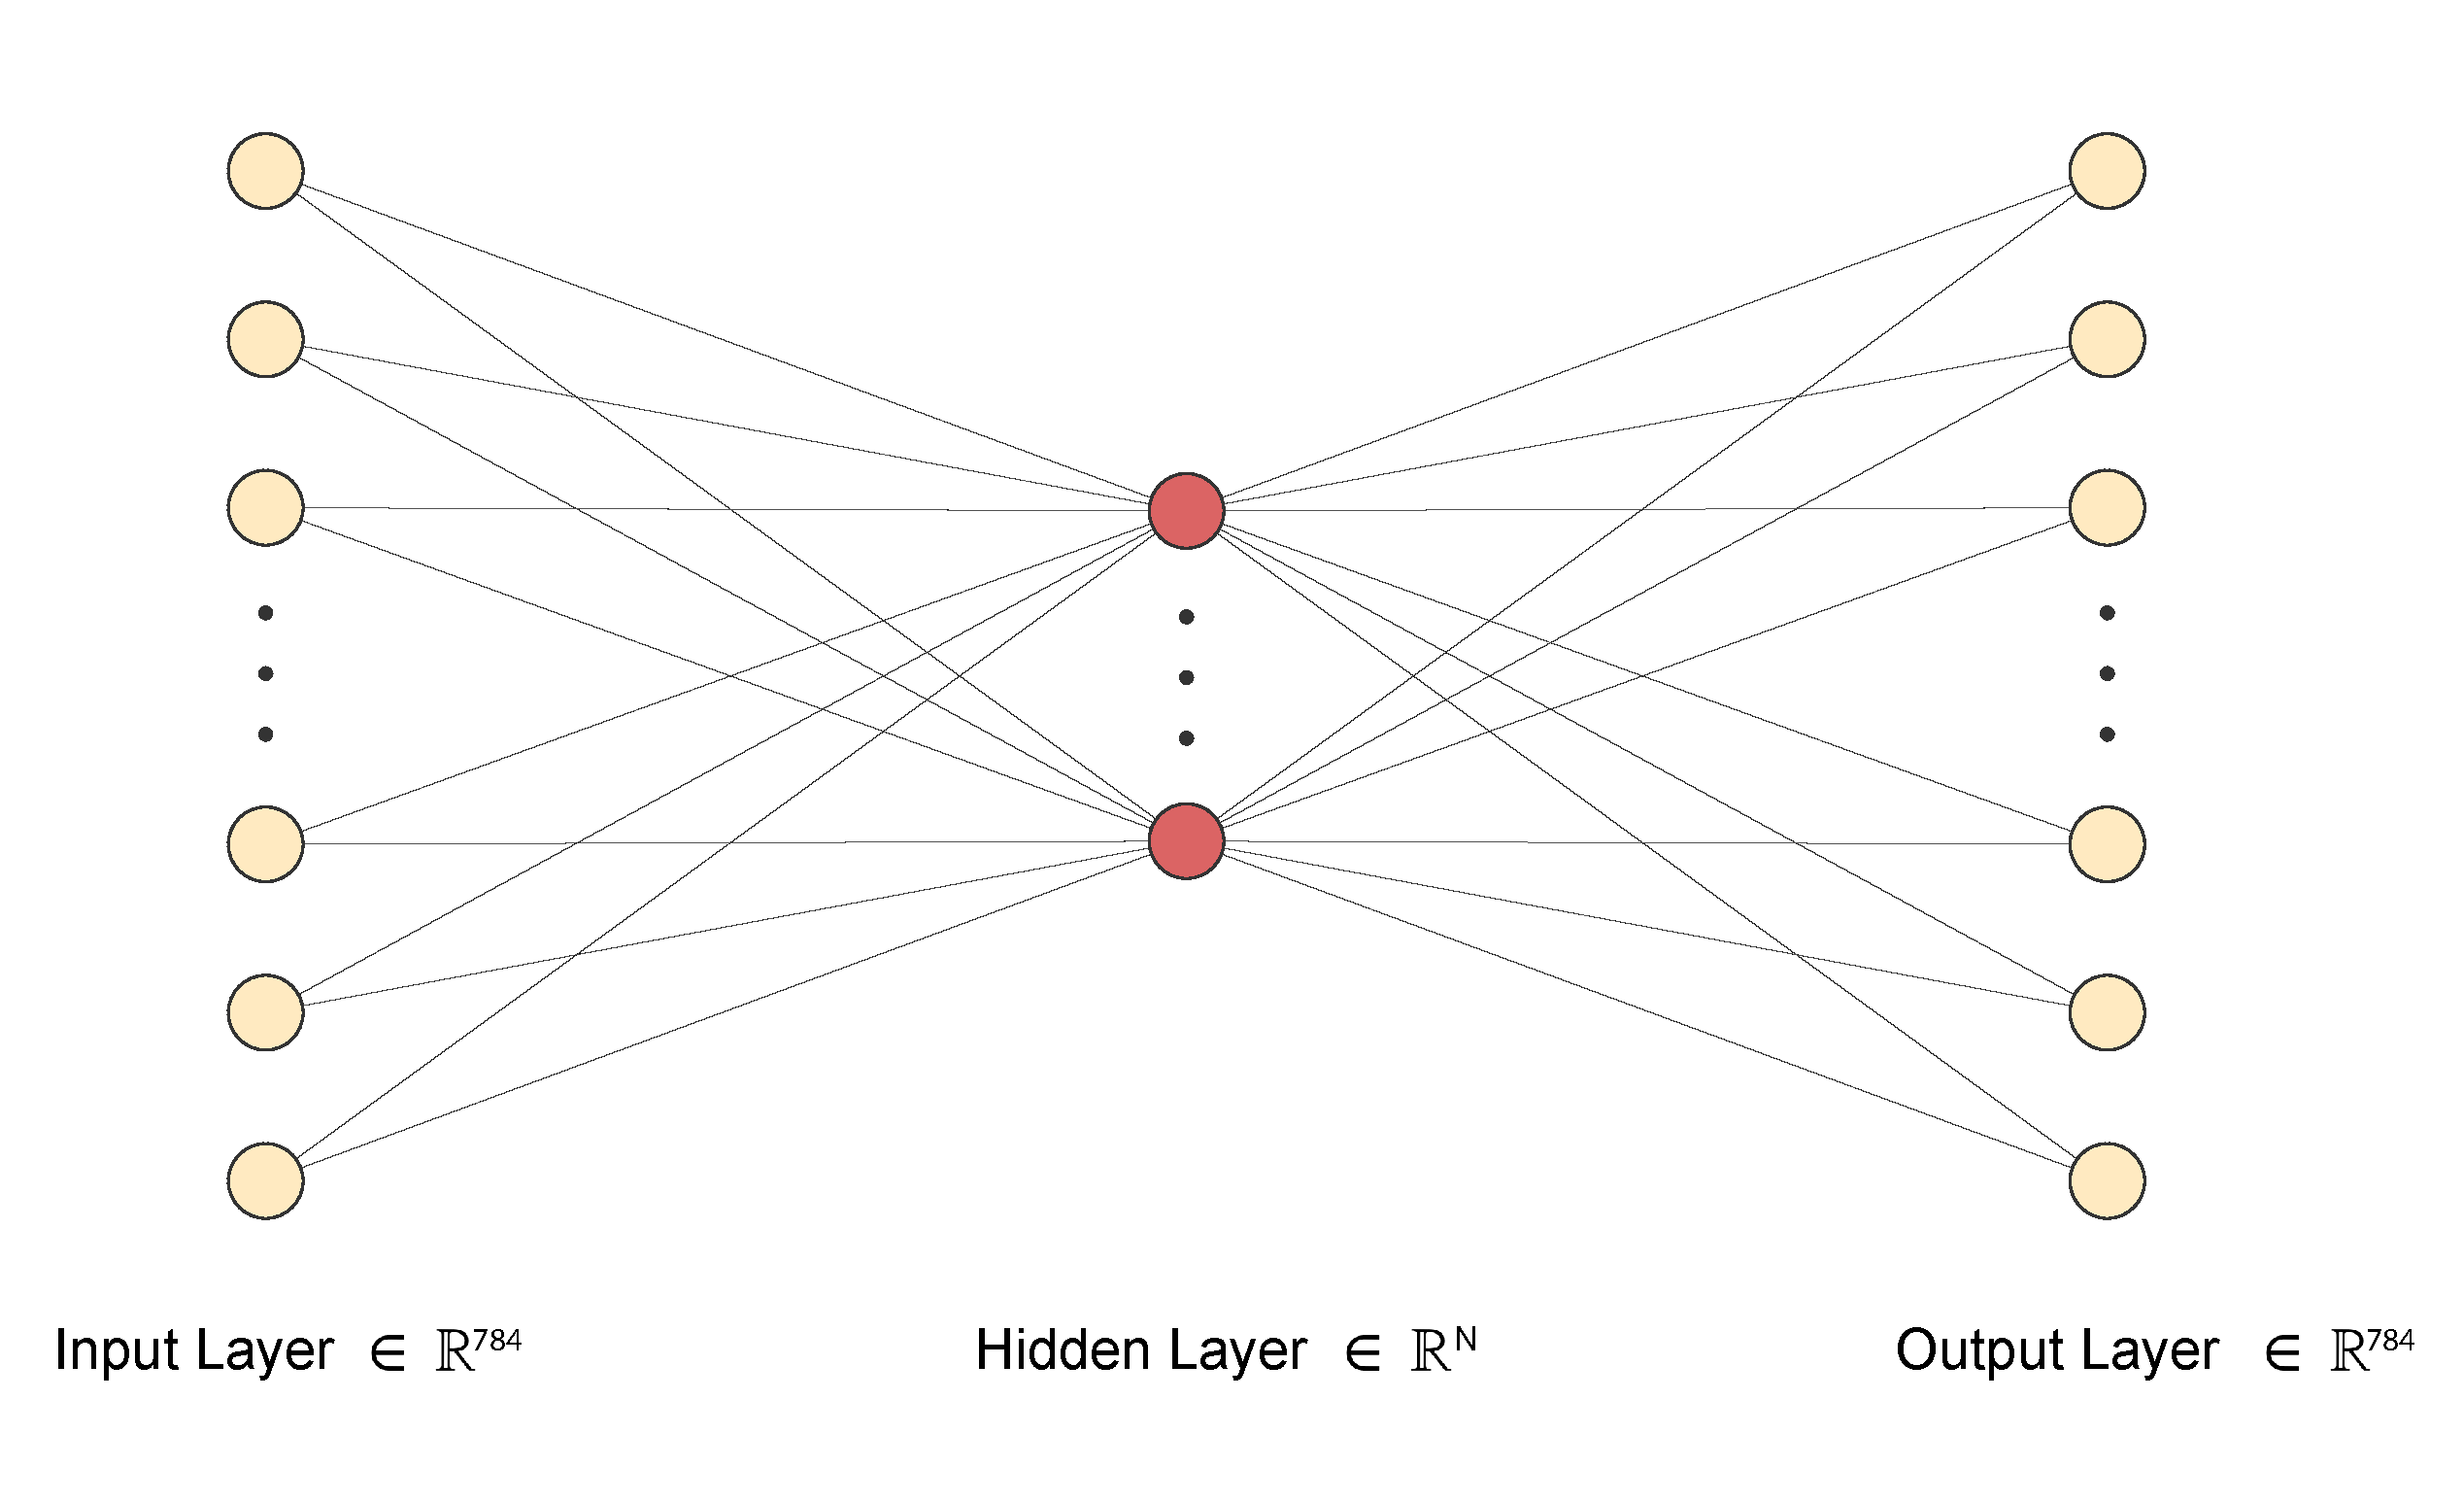
\includegraphics[width=1.0\textwidth]{graphics/autoencoder_diagram.pdf}
    \textbf{Notes}: Input and output layers each contain 784 nodes respectively, in congruence with the dimensions of MNIST image instance vectors. Intermediate nodes are omitted for ease of interpretability. Hidden layers contain a variable number of nodes, $N$, varied across seven values: 2, 4, 8, 14, 28, 56, and 112. Encoding of inputs occurs through weighting of activations between input and hidden layers. Image reconstruction occurs through weighting of activations between hidden and output layers.
\end{figure}

\begin{figure}
    \caption{Generic autoencoder architecture, with bias}
	\label{fig:autoencoder-diagram-bias}
	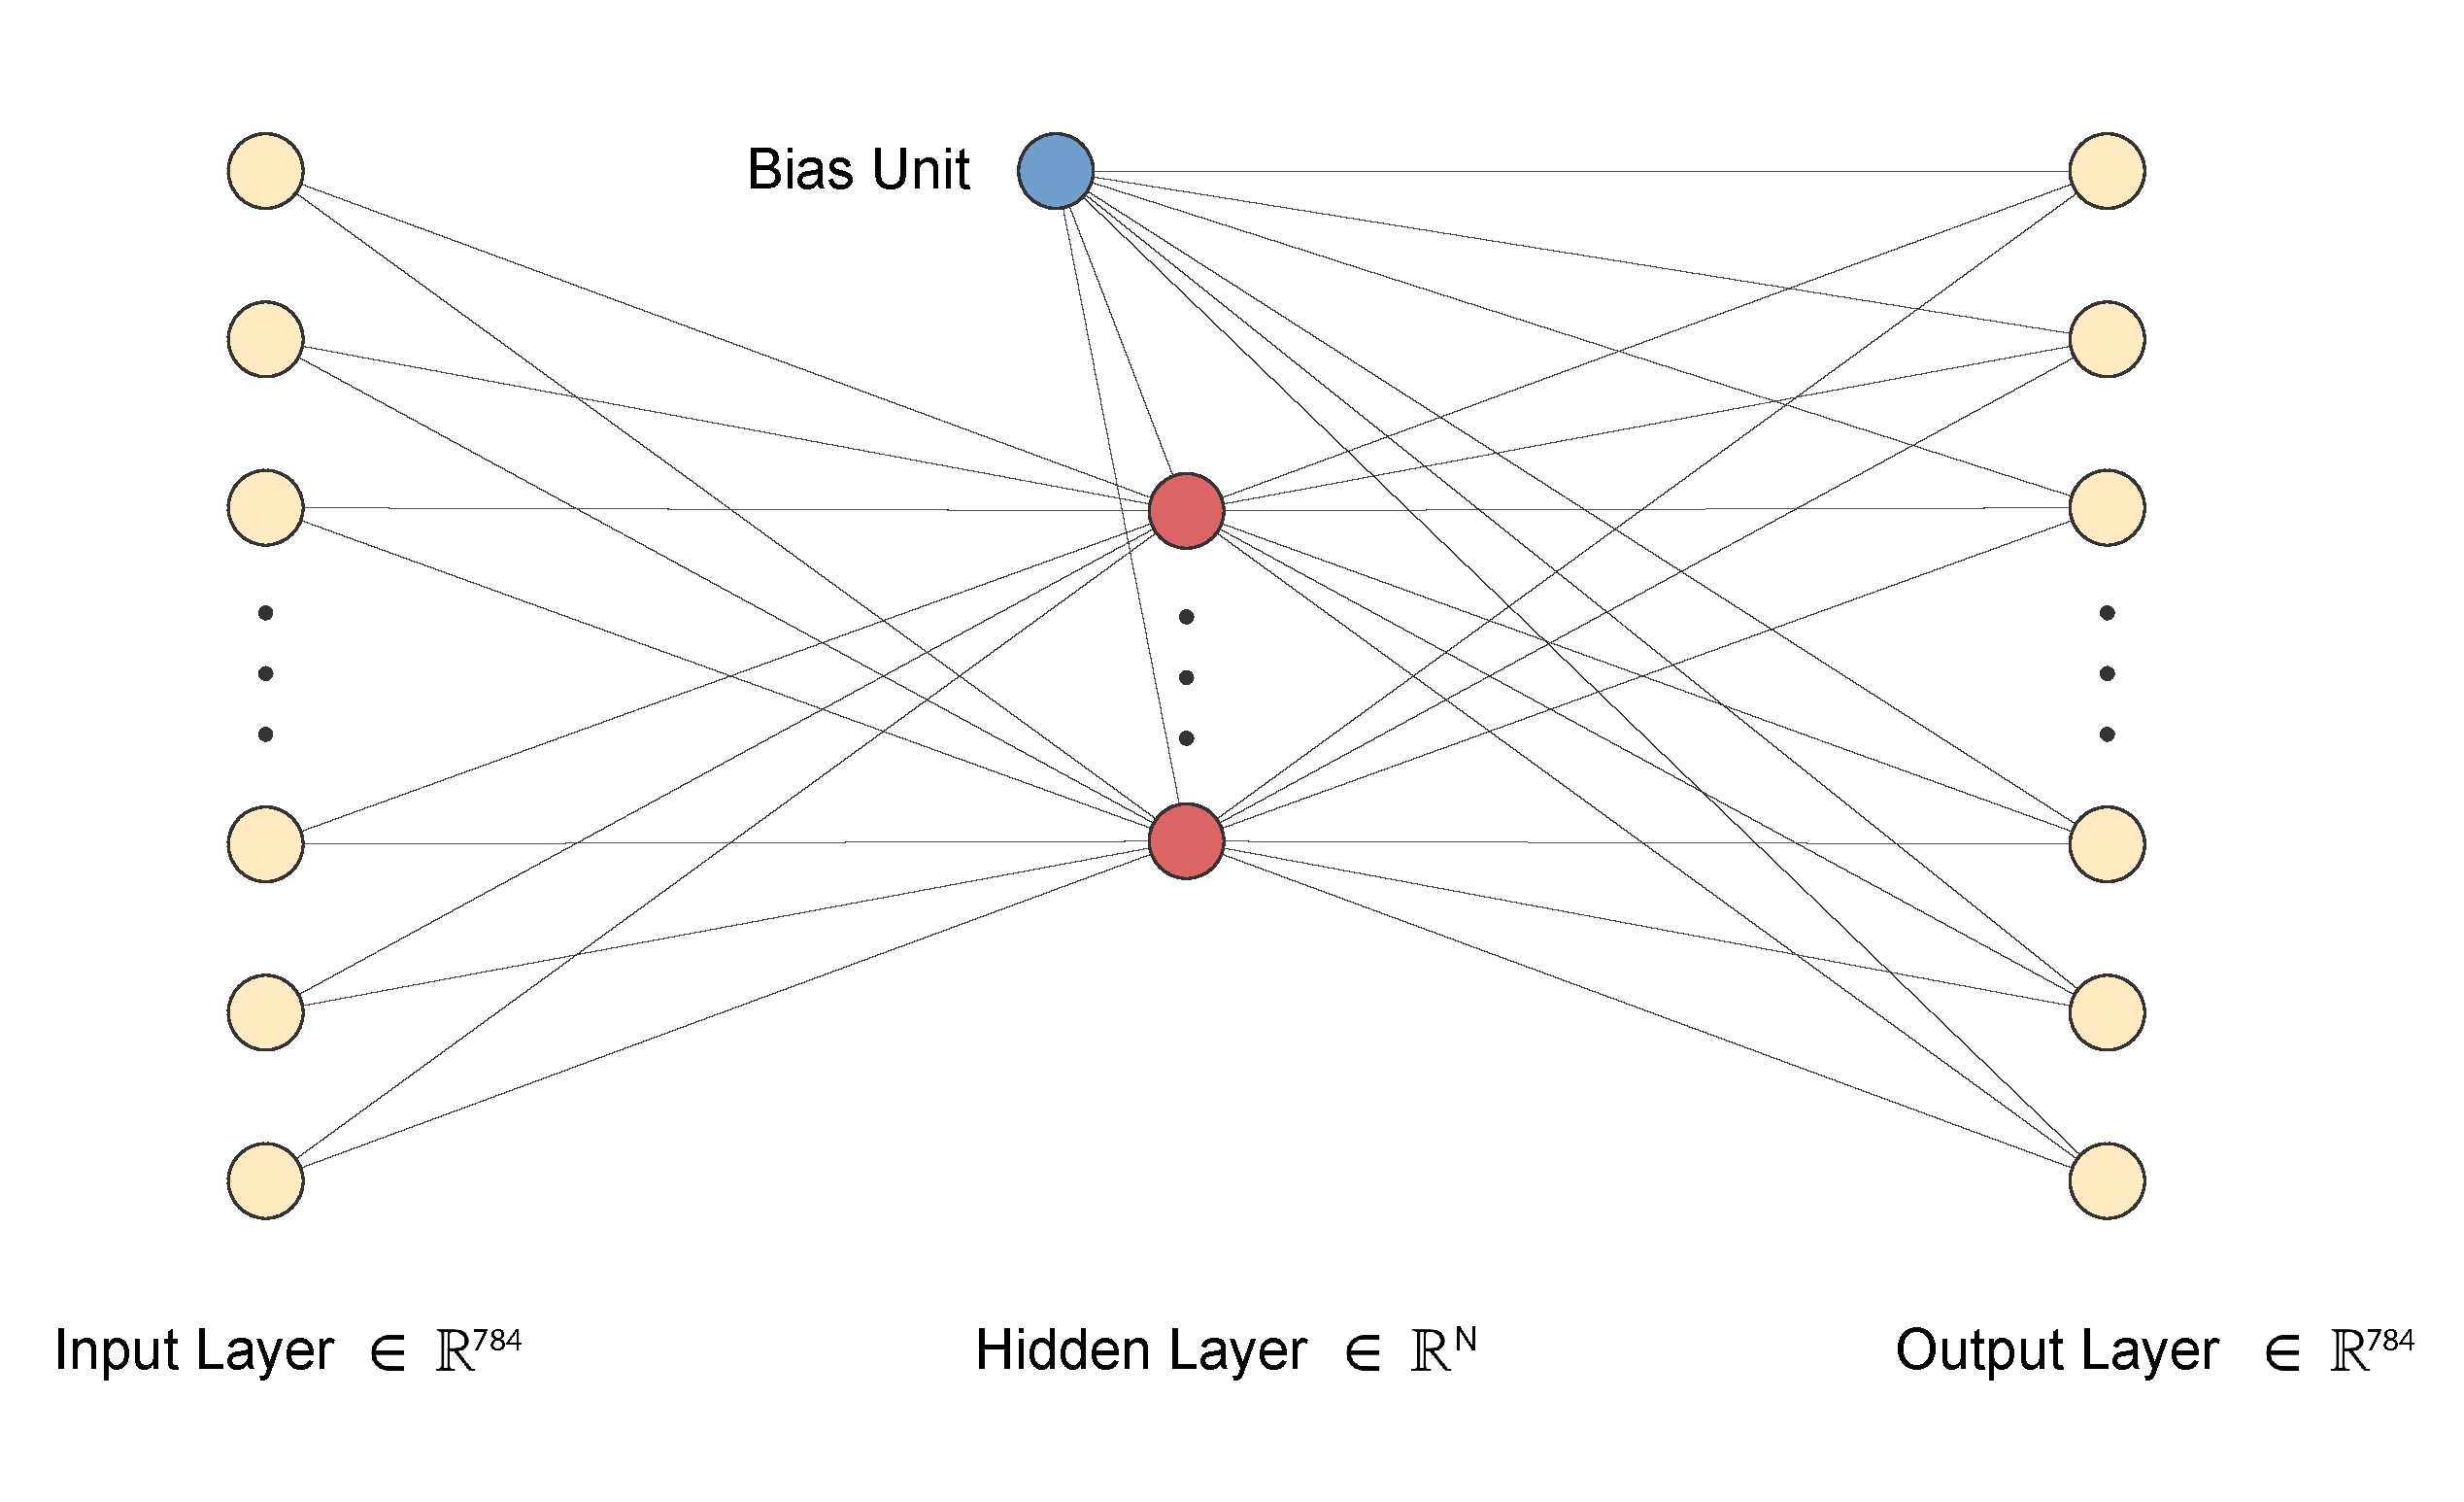
\includegraphics[width=1.0\textwidth]{graphics/autoencoder_diagram_bias.pdf}
    \textbf{Notes}: Input and output layers each contain 784 nodes respectively, in congruence with the dimensions of MNIST image instance vectors. Intermediate nodes are omitted for ease of interpretability. Hidden layers contain a variable number of nodes, $N$, varied across seven values: 2, 4, 8, 14, 28, 56, and 112. A  constant bias affects activations in hidden and output nodes differentially through learned bias weights. Encoding of inputs occurs through weighting of activations between input and hidden layers. Image reconstruction occurs through weighting of activations between hidden and output layers. 
\end{figure}

\begin{figure}
    \caption{Reconstruction mean-squared error throughout training phase, disaggregated by network architecture}
	\label{fig:training-loss}
	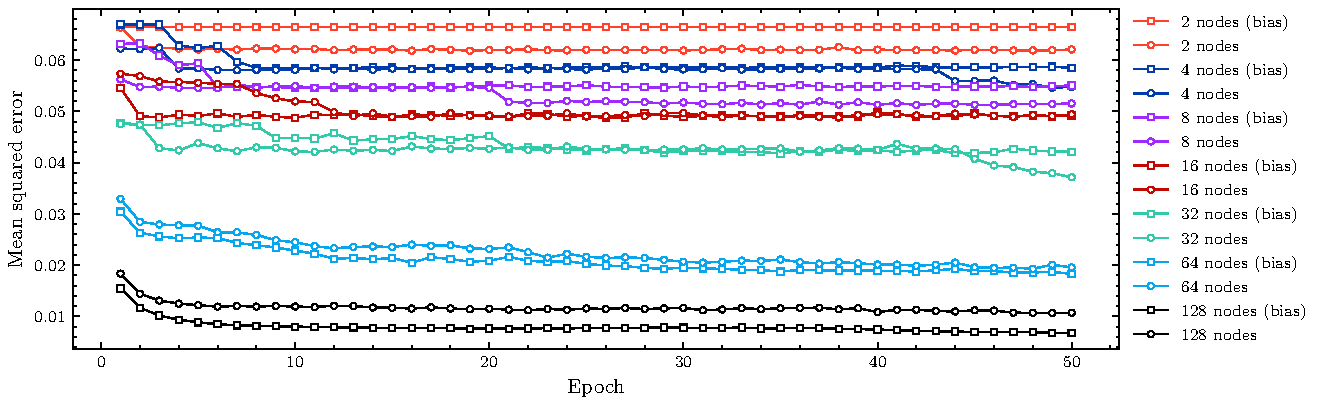
\includegraphics[width=1.0\textwidth]{graphics/model_loss.pdf}
    \textbf{Notes}: Mean-squared error (MSE) of autoencoder networks across validation partition of MNIST dataset. MSE was calculated through forward propogation of MNIST validation instances (N=10,000) using trained weights at each discrete training timestep. Learning rate for each model was set at 0.01.
\end{figure}